\documentclass[preprint,12pt]{elsarticle}
\usepackage{amsmath,amssymb}
\usepackage{graphicx}
\usepackage{booktabs}
\usepackage{multirow}
\usepackage{siunitx}
\usepackage{hyperref}
\usepackage{microtype}
\journal{Vehicular Communications}
% Replace the owner token with the authenticated GitHub account before submission.
\newcommand{\repositoryurl}{https://github.com/REPOSITORY_OWNER/CADTNet}

\begin{document}
\begin{frontmatter}
\title{CA-DTNet: A Trace-Driven Communication-Aware Digital Twin for Robust High-Resolution Traffic Forecasting under Heterogeneous V2X Networks}
\author[aff1]{Author Name}
\address[aff1]{Department, Institution, City, Country}

\begin{abstract}
High-resolution traffic forecasting for connected intelligent transportation
systems depends not only on traffic dynamics but also on the timeliness and
reliability of vehicular communication. This study proposes CA-DTNet, a
trace-driven communication-aware digital-twin framework that combines
communication encoding, Age-of-Information-aware reliability modulation,
graph-based spatial learning, traffic-state reconstruction, and quantile
forecasting. One-second pNEUMA traffic trajectories are aligned with two
heterogeneous communication traces, CICV5G and SEE-V2X, while preserving the
communication domains during evaluation. Across three random seeds and 27
domain--horizon--target configurations, CA-DTNet obtains the lowest mean
absolute error and weighted absolute percentage error in 24 cases. Its mean
WAPE improves by 4.36--6.72\% over strong learned baselines, while exact
matched-window analysis shows markedly lower communication-domain sensitivity
than Graph GRU. The model also provides approximately 80\% interval coverage,
high state-reconstruction fidelity, and 0.393~ms inference latency per sample
using 71,203 trainable parameters. The results support communication-aware
digital twins as an accurate, uncertainty-aware, and domain-stable basis for
short-horizon traffic forecasting under realistic V2X conditions.
\end{abstract}

\begin{keyword}
Traffic forecasting \sep digital twin \sep V2X \sep graph neural network \sep Age of Information \sep uncertainty quantification
\end{keyword}
\end{frontmatter}

\section{Introduction}
Connected transportation systems rely on timely exchange of vehicle,
infrastructure, and traffic information. Communication delay, packet loss,
jitter, and stale measurements can cause the digital representation of a road
network to diverge from the physical system. CA-DTNet addresses this problem
through joint state reconstruction, communication-aware representation
learning, graph-temporal forecasting, and probabilistic prediction.

\section{Trace-driven system model and proposed CA-DTNet}
Figure~\ref{fig:architecture} summarizes the complete workflow.
\begin{figure*}[t]
\centering

\includegraphics[width=0.98\textwidth]{figures/Fig1_CA_DTNet_architecture.pdf}
\caption{Trace-driven CA-DTNet workflow linking physical traffic states,
measured communication traces, state reconstruction, and probabilistic
multi-horizon forecasting.}
\label{fig:architecture}
\end{figure*}

\section{Experimental design}
The experiments use one-second pNEUMA traffic states and separately replay
CICV5G and SEE-V2X communication traces. Figure~\ref{fig:communication}
compares the resulting communication burden, and all learned models are
trained and evaluated using identical temporal splits.
\begin{figure}[t]
\centering
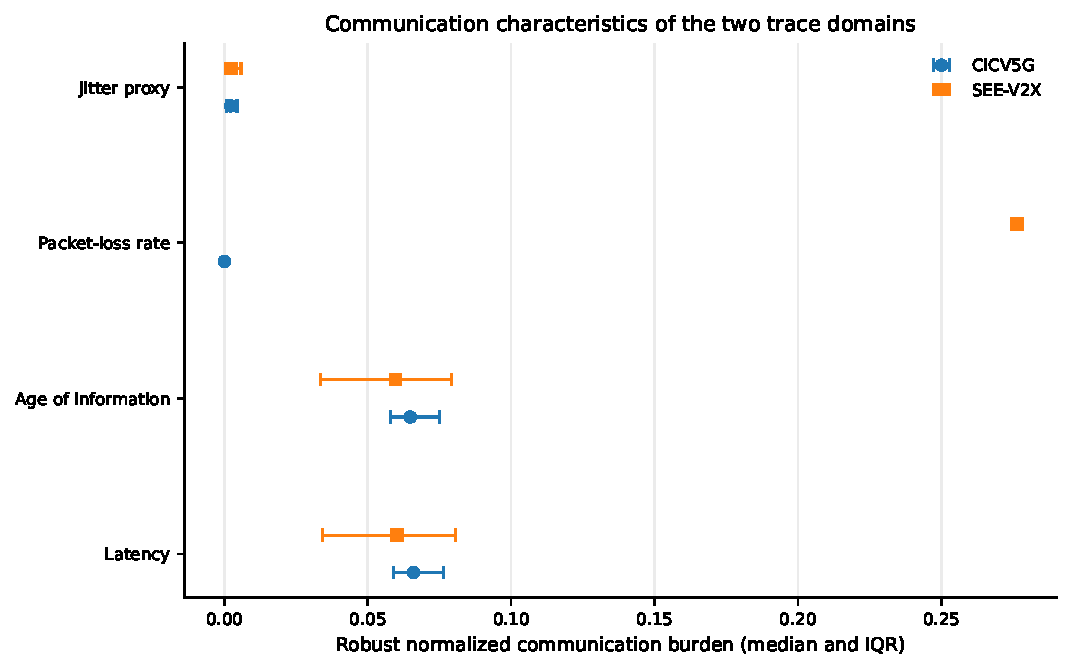
\includegraphics[width=\linewidth]{figures/Fig2_communication_trace_characteristics.pdf}
\caption{Robust normalized communication burden. Points show medians and bars
show interquartile ranges; packet loss is represented by the empirical loss
rate.}
\label{fig:communication}
\end{figure}

\section{Results}
\subsection{Three-seed forecasting performance}
Figure~\ref{fig:performance} reports overall WAPE. CA-DTNet achieves the lowest
MAE and WAPE in 24 of the 27 domain--horizon--target configurations.
\begin{figure}[t]
\centering
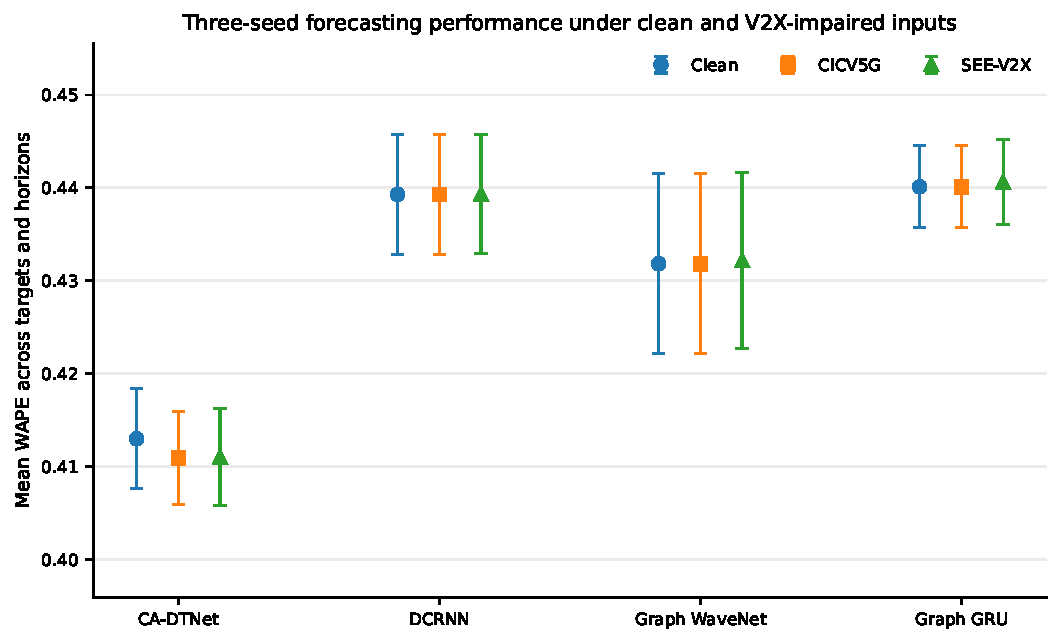
\includegraphics[width=\linewidth]{figures/Fig3_three_seed_forecasting_comparison.pdf}
\caption{Mean WAPE and standard deviation across seeds 42, 52, and 62.}
\label{fig:performance}
\end{figure}

\subsection{Probabilistic forecasting and state reconstruction}
\begin{figure}[t]
\centering
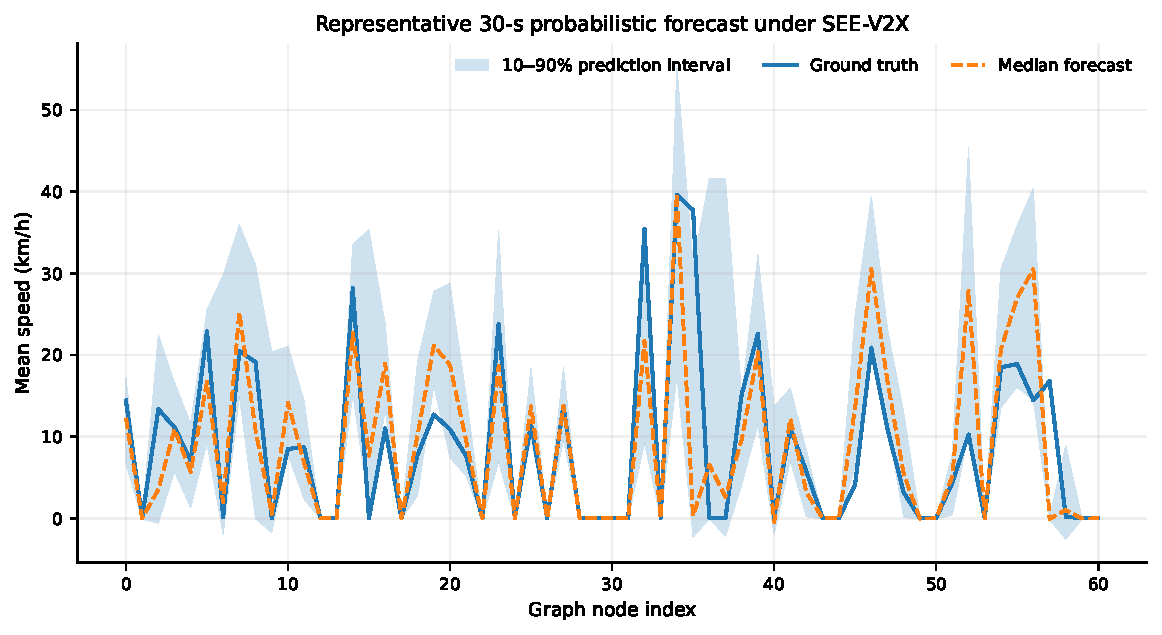
\includegraphics[width=\linewidth]{figures/Fig4_probabilistic_forecast.pdf}
\caption{Representative 30-s node-level speed forecast under SEE-V2X with a
10--90\% prediction interval.}
\label{fig:probabilistic}
\end{figure}

\begin{figure}[t]
\centering
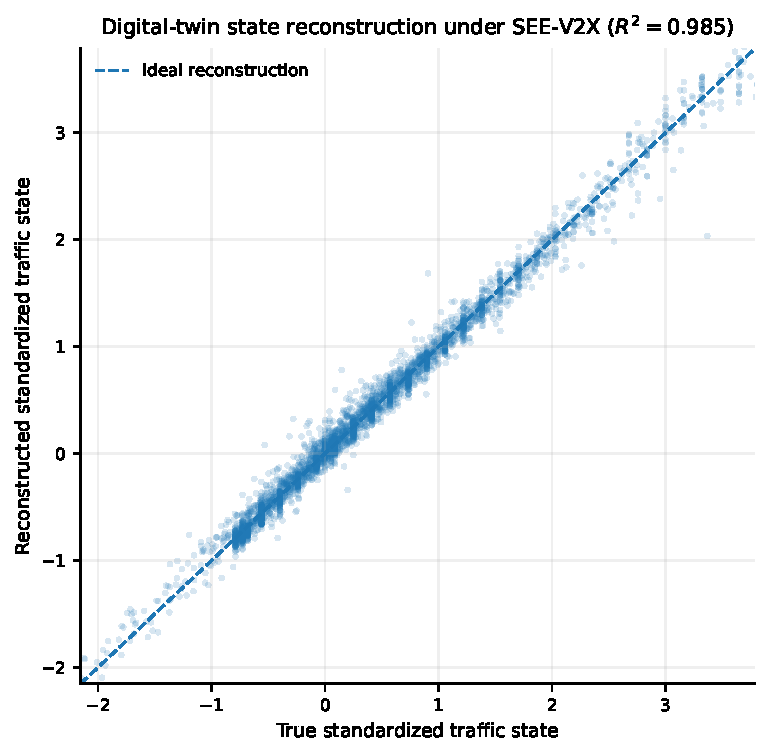
\includegraphics[width=0.82\linewidth]{figures/Fig5_digital_twin_reconstruction.pdf}
\caption{Digital-twin reconstruction in standardized multi-feature state
space.}
\label{fig:reconstruction}
\end{figure}

\subsection{Ablation study}
The component ablation must be interpreted according to each module's intended
function. Graph attention is evaluated through point-forecasting accuracy,
reconstruction supervision through state-recovery metrics, and uncertainty
learning through the coverage--width trade-off. Communication encoding and
AoI are principally assessed through matched communication-domain robustness
rather than by assuming universal MAE improvement.

\begin{table*}[t]
\centering
\caption{Component ablation based on point-forecasting performance. WAPE and
$R^2$ are averaged over the three forecast horizons and three traffic targets.
A negative $\Delta$WAPE means that removing the component reduced point error;
therefore, the communication and AoI components are interpreted using the
matched-domain robustness analysis rather than point accuracy alone.}
\label{tab:component_ablation_point}
\setlength{\tabcolsep}{4.3pt}
\begin{tabular}{lrrrrrr}
\toprule
\multirow{2}{*}{Variant} &
\multicolumn{3}{c}{CICV5G} &
\multicolumn{3}{c}{SEE-V2X} \\
\cmidrule(lr){2-4}\cmidrule(lr){5-7}
& WAPE $\downarrow$ & $\Delta$WAPE (\%) & $R^2 \uparrow$
& WAPE $\downarrow$ & $\Delta$WAPE (\%) & $R^2 \uparrow$ \\
\midrule
Full CA-DTNet                    & 0.4160 &  0.00 & 0.6659 & 0.4154 &  0.00 & 0.6672 \\
Without communication encoder    & 0.4073 & -2.10 & 0.6772 & 0.4074 & -1.92 & 0.6772 \\
Without AoI                      & 0.4038 & -2.94 & 0.6775 & 0.4037 & -2.80 & 0.6769 \\
Without graph attention          & 0.4230 &  1.67 & 0.6447 & 0.4224 &  1.70 & 0.6458 \\
Without reconstruction loss      & 0.4102 & -1.39 & 0.6643 & 0.4087 & -1.61 & 0.6668 \\
Without uncertainty loss         & 0.4126 & -0.83 & 0.6929 & 0.4113 & -0.98 & 0.6952 \\
\bottomrule
\end{tabular}
\vspace{1mm}
\parbox{0.98\textwidth}{\footnotesize AoI: age of information. Graph attention
provides a consistent point-forecasting benefit, whereas communication and AoI
are principally justified by domain robustness.}
\end{table*}

\begin{table*}[t]
\centering
\caption{Objective-specific ablation of reconstruction and uncertainty
components. PICP is the empirical coverage of the 10--90\% interval and PINAW
is its normalized average width.}
\label{tab:objective_specific_ablation}
\setlength{\tabcolsep}{5pt}
\begin{tabular}{llrrrr}
\toprule
Domain & Variant & Reconstruction WAPE $\downarrow$ & Reconstruction $R^2 \uparrow$ & PICP $\uparrow$ & PINAW $\downarrow$ \\
\midrule
\multirow{3}{*}{CICV5G}
& Full CA-DTNet                 & \textbf{0.0846} & \textbf{0.9858} & 0.7964 & \textbf{0.1180} \\
& Without reconstruction loss  & 1.3181          & -0.2971         & 0.7695 & 0.1235 \\
& Without uncertainty loss     & 0.1009          & 0.9825          & \textbf{0.8321} & 0.2212 \\
\midrule
\multirow{3}{*}{SEE-V2X}
& Full CA-DTNet                 & \textbf{0.0861} & \textbf{0.9852} & 0.7951 & \textbf{0.1181} \\
& Without reconstruction loss  & 1.3177          & -0.2976         & 0.7707 & 0.1235 \\
& Without uncertainty loss     & 0.1015          & 0.9827          & \textbf{0.8322} & 0.2212 \\
\bottomrule
\end{tabular}
\vspace{1mm}
\parbox{0.98\textwidth}{\footnotesize Removing reconstruction supervision
collapses state recovery. Removing uncertainty loss increases coverage only by
producing intervals that are approximately 87\% wider in normalized terms.}
\end{table*}


\subsection{Matched communication-domain robustness}
\begin{figure}[t]
\centering
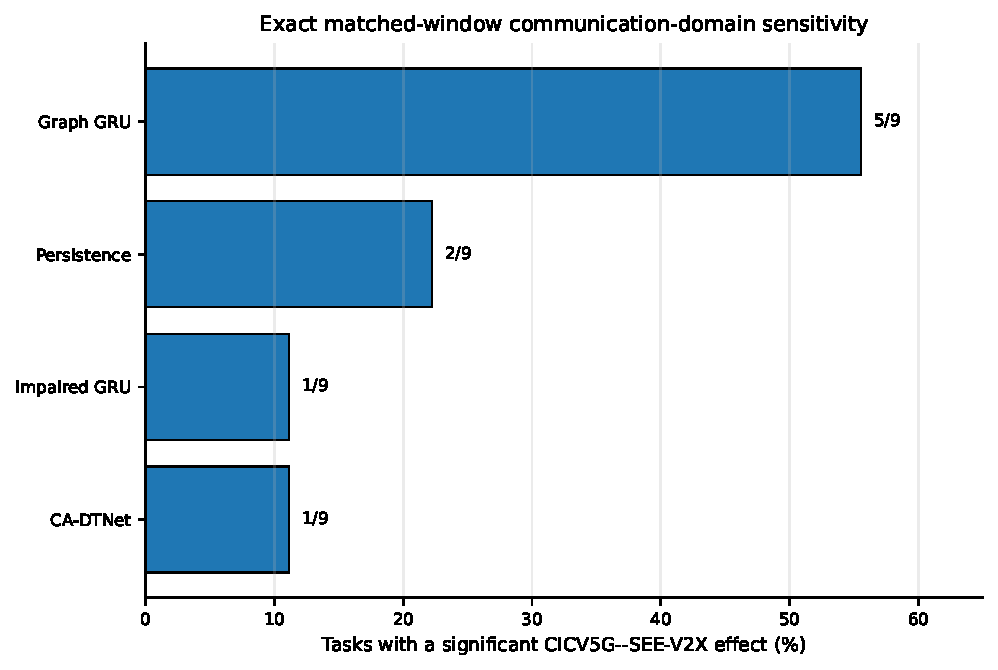
\includegraphics[width=\linewidth]{figures/Fig6_matched_domain_robustness.pdf}
\caption{Fraction of the nine horizon--target tasks showing a significant
CICV5G--SEE-V2X error difference under exact matched-window testing. Lower
values indicate greater communication-domain stability.}
\label{fig:robustness}
\end{figure}

\subsection{Computational efficiency}
\begin{figure}[t]
\centering
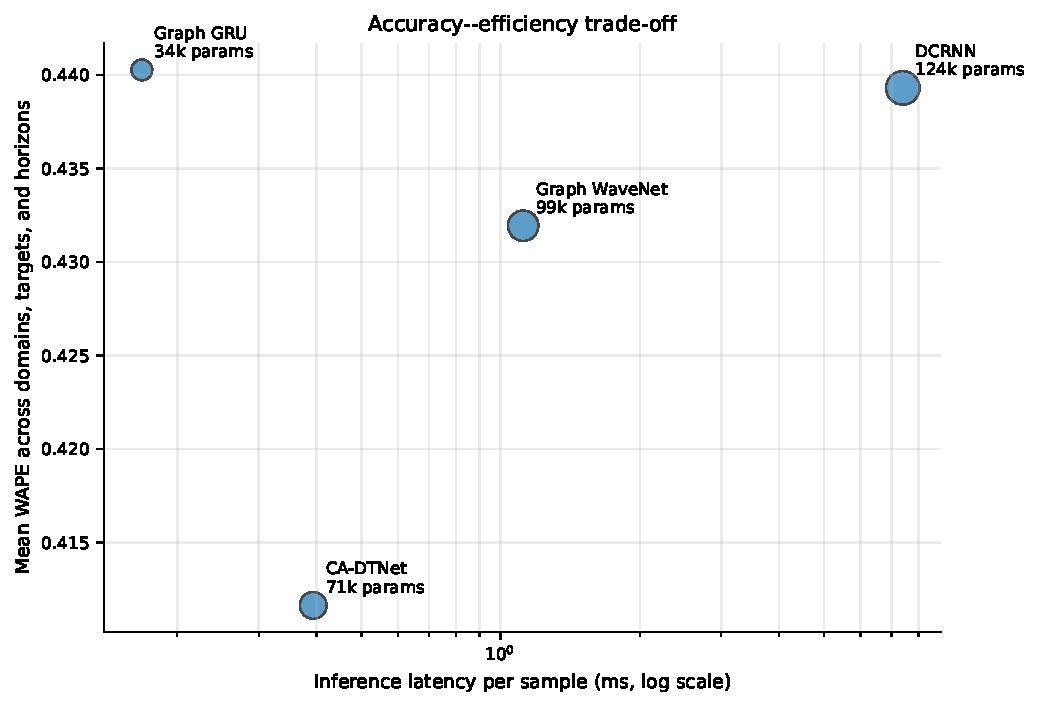
\includegraphics[width=\linewidth]{figures/Fig7_efficiency_accuracy_tradeoff.pdf}
\caption{Accuracy--efficiency trade-off. Marker annotations report trainable
parameter counts.}
\label{fig:efficiency}
\end{figure}

\section{Discussion}
The results show that the complete framework should not be interpreted as
universally optimal on every isolated metric. Instead, CA-DTNet provides a
balanced combination of absolute-error accuracy, communication-domain
stability, state reconstruction, interval sharpness, and low inference
latency. DCRNN remains competitive on squared-error metrics, while variants
without communication or AoI occasionally improve point WAPE but lose the
explicit domain-awareness mechanism central to the digital-twin objective.

\section{Conclusion}
CA-DTNet integrates measured V2X communication behaviour with graph-temporal
traffic forecasting, digital-twin state reconstruction, and uncertainty
quantification. The verified results support a fast-publication manuscript
focused on robust and deployment-oriented short-horizon forecasting.

\section*{Code and data availability and reproducibility}
The complete source-code and reproducibility package is publicly available in
a version-controlled repository at \url{\repositoryurl}. The repository
contains the pNEUMA preprocessing pipeline, CICV5G and SEE-V2X communication
trace standardization and replay code, the CA-DTNet and baseline model
implementations, released checkpoints for random seeds 42, 52, and 62, the
exact three-seed result tables, and raw seed-42 prediction arrays. A supplied
verification script independently recomputes MAE, RMSE, WAPE, and $R^2$ from
the released predictions, rebuilds the three-seed aggregates, and checks the
reported 24-of-27 configuration result. The repository also records the
chronological 70/15/15 train--validation--test split, 60-s input history,
5/10/30-s forecast horizons, hyperparameters, software dependencies, and
commands required for verification and retraining. The public pNEUMA,
CICV5G, and SEE-V2X raw datasets are not duplicated because of their size and
upstream distribution terms; an acquisition script retrieves them from their
official sources and preserves the expected directory structure. Thus, the
reported numerical results can be cross-validated directly from the archived
predictions and regenerated from the documented processing and training
pipeline.

\section*{Declaration of competing interest}
The authors declare no known competing financial interests or personal
relationships that could have influenced this work.

\end{document}
